\documentclass[czech, kiv, ba, he, iso690numb, pdf]{fasthesis}

\usepackage{url}
\usepackage{enumitem}

\lstdefinelanguage{json}{
    basicstyle=\ttfamily\small,
    showstringspaces=false,
    backgroundcolor=\color{white},
    literate=
     *{0}{{{\color{blue}0}}}{1}
      {1}{{{\color{blue}1}}}{1}
      {2}{{{\color{blue}2}}}{1}
      {3}{{{\color{blue}3}}}{1}
      {4}{{{\color{blue}4}}}{1}
      {5}{{{\color{blue}5}}}{1}
      {6}{{{\color{blue}6}}}{1}
      {7}{{{\color{blue}7}}}{1}
      {8}{{{\color{blue}8}}}{1}
      {9}{{{\color{blue}9}}}{1}
      {:}{{{\color{red}:}}}{1}
      {,}{{{\color{red},}}}{1}
      {\{}{{{\color{black}\{}}}{1}
      {\}}{{{\color{black}\}}}}{1}
      {[}{{{\color{black}[}}}{1}
      {]}{{{\color{black}]}}}{1},
}

\title{Implementace modulu pro import údajů RÚIAN}
\author{Martin}{Schön}{}{}
\supervisor{Martin Bíkl, Ing. Petr Přibyl, Ing. Martin Zíma Ph.D.}
\stagworkid{100718}
\assignment{figures/zadani.pdf}
\signdate{31}{12}{2024}{V Plzni}
\addbibresource{bib.bib}
\abstract{Text abstraktu v~jazyce práce, tj. zde česky.}
{The abstract text in a secondary language, here in English.}
\keywords{}
\acknowledgement{Text poděkování.}

\begin{document}
\frontpages[tm]
\tableofcontents
%---------------------------------------------------------------------------

Problematika správy uzemní identifikace a prostorových dat a~jejich synchronizace mezi různými systémy
nabývá na významu s~rostoucí digitalizací státní správy a~soukromých sektorů.
Jedním z~klíčových zdrojů těchto dat v~České republice je Registr územní identifikace,
adres a~nemovitostí (RÚIAN), který poskytuje rozsáhlé a~aktuální informace o~územních
objektech, adresách a~dalších klíčových entitách. Efektivní využití dat z~RÚIAN vyžaduje
nejen jejich přístup prostřednictvím datových služeb, ale také robustní řešení pro mapování,
konfiguraci a~synchronizaci datových struktur.

Cílem této bakalářské práce je analyzovat datové schéma registru RÚIAN a~možnosti získávání
dat prostřednictvím nabízených datových služeb. Dále bude provedena analýza a~návrh konfiguračního
řešení, které umožní nastavit úroveň přenášených územních objektů a~cílové databázové struktury.
V~rámci práce bude navržena a~implementována aplikace, která umožní pravidelnou synchronizaci dat
z~veřejné databáze RÚIAN do cílových databázových struktur s~podporou databází Oracle,
Microsoft~SQL Server a~PostgreSQL. Aplikace bude schopna provádět synchronizaci kompletních datových
sad i~přírůstkových změn podle zadané konfigurace.
RÚIAN je zkratkou pro Registr územní identifikace, adres a~nemovitostí.
Jedná se o~státní informační systém v~České republice, který obsahuje informace o~adresách, budovách, parcelách a~dalších objektech.
Systém je spravován Českým úřadem zeměměřickým a~katastrálním (ČÚZK).
Data jsou využívána v~mnoha oblastech, například v~urbanistickém plánování, geodézii nebo při správě nemovitostí.
Jednotlivé prvky jsou zobrazovány na~mapách státního mapového díla a~digitální mapě veřejné správy.

Data z~RÚIAN jsou veřejně dostupná a~lze je získat z~webové služby na~adrese \url{https://vdp.cuzk.gov.cz/vdp/ruian}.
Lze stahovat data ve~formátu XML, která obsahují základní nebo úplné informace o~územních prvcích.
Mezi tyto prvky patří Stát, VÚSC (Vyšší územní samosprávný celek), ORP (Obec s~rozšířenou působností), Obec, Část obce, Ulice, Adresa atd.
Data lze vyhledávat, ověřovat a~stahovat dle jednotlivých územních prvků, které jsou uloženy v~databázi RÚIAN.

\section{Výměnný formát RÚIAN}
Výměnný formát RÚIAN (VFR) je jednou ze služeb, které poskytuje ČÚZK.
Tento formát slouží k~přenosu dat mezi různými informačními systémy.

Je možné stahovat data podle zadaných formátů: \textbf{Standardní}, \textbf{Historický} a~\textbf{Speciální}.
Dále je možné si vybrat mezi přírůstkovými daty a~úplnou kopií.
Přírůstky je možné vyhledávat podle data -- od~zvoleného dne až do~současnosti.
Úplná kopie obsahuje všechna data a~je možné ji také časově vymezit. Tato data se aktualizují jednou měsíčně.

Každý formát navíc nabízí další parametry, které lze nastavit.
Data z~VFR jsou ve~formátu XML.
Každý XML element obsahuje atributy, které nesou informace o~dané entitě (tabulce).

\newpage

\begin{itemize}
    \item \textbf{Standardní} -- obsahuje úplná nebo přírůstková data.
    \begin{itemize}[itemsep=0pt]
        \item Časový rozsah: přírůstky od~data / úplná kopie,
        \item Územní prvky: Stát až~ZSJ / Obec a~podřazené,
        \item Datová sada: základní / kompletní,
        \item Výběr údajů: základní údaje / generované hranice, originální hranice, vlajky a~znaky,
        \item Územní omezení: ČR / kraj (VÚSC) / ORP / obec,
    \end{itemize}

    \item \textbf{Historický} -- obsahuje historická data.
    \begin{itemize}[itemsep=0pt]
        \item Časový rozsah: přírůstky od~data / úplná kopie,
        \item Územní prvky: Stát až~ZJS / Obec a~podřazené,
        \item Územní omezení: ČR / kraj (VÚSC) / ORP / obec,
    \end{itemize}

    \item \textbf{Speciální} -- obsahuje speciální datové sady.
    \begin{itemize}[itemsep=0pt]
        \item Časový rozsah: přírůstky od~data / úplná kopie,
        \item Výběr údajů: číselníky / vazby / vazby a~číselníky,
        \item Kategorie: všechny / geodetické body / nerostné bohatství,
    \end{itemize}
\end{itemize}

\section{Datové struktury}
Data z~RÚIAN jsou rozdělena do~několika datových struktur neboli entit.
Jak je vidět na obrázku~\ref{fig:ruian_tables} \cite{ruian_vfr}, každá entita obsahuje specifické informace.
Mezi tyto informace patří například název státu, kód státu, geografické souřadnice, datum vzniku a~další. 

Stát představuje nejvyšší úroveň hierarchie, pod kterou spadají další entity závislé na~ní.
Příkladem je entita \textbf{VÚSC}, která obsahuje informace o~vyšších územních samosprávných celcích.
Jednotlivé entity na~sebe navzájem odkazují pomocí cizích klíčů.

\begin{figure}[!h]
    \centering
    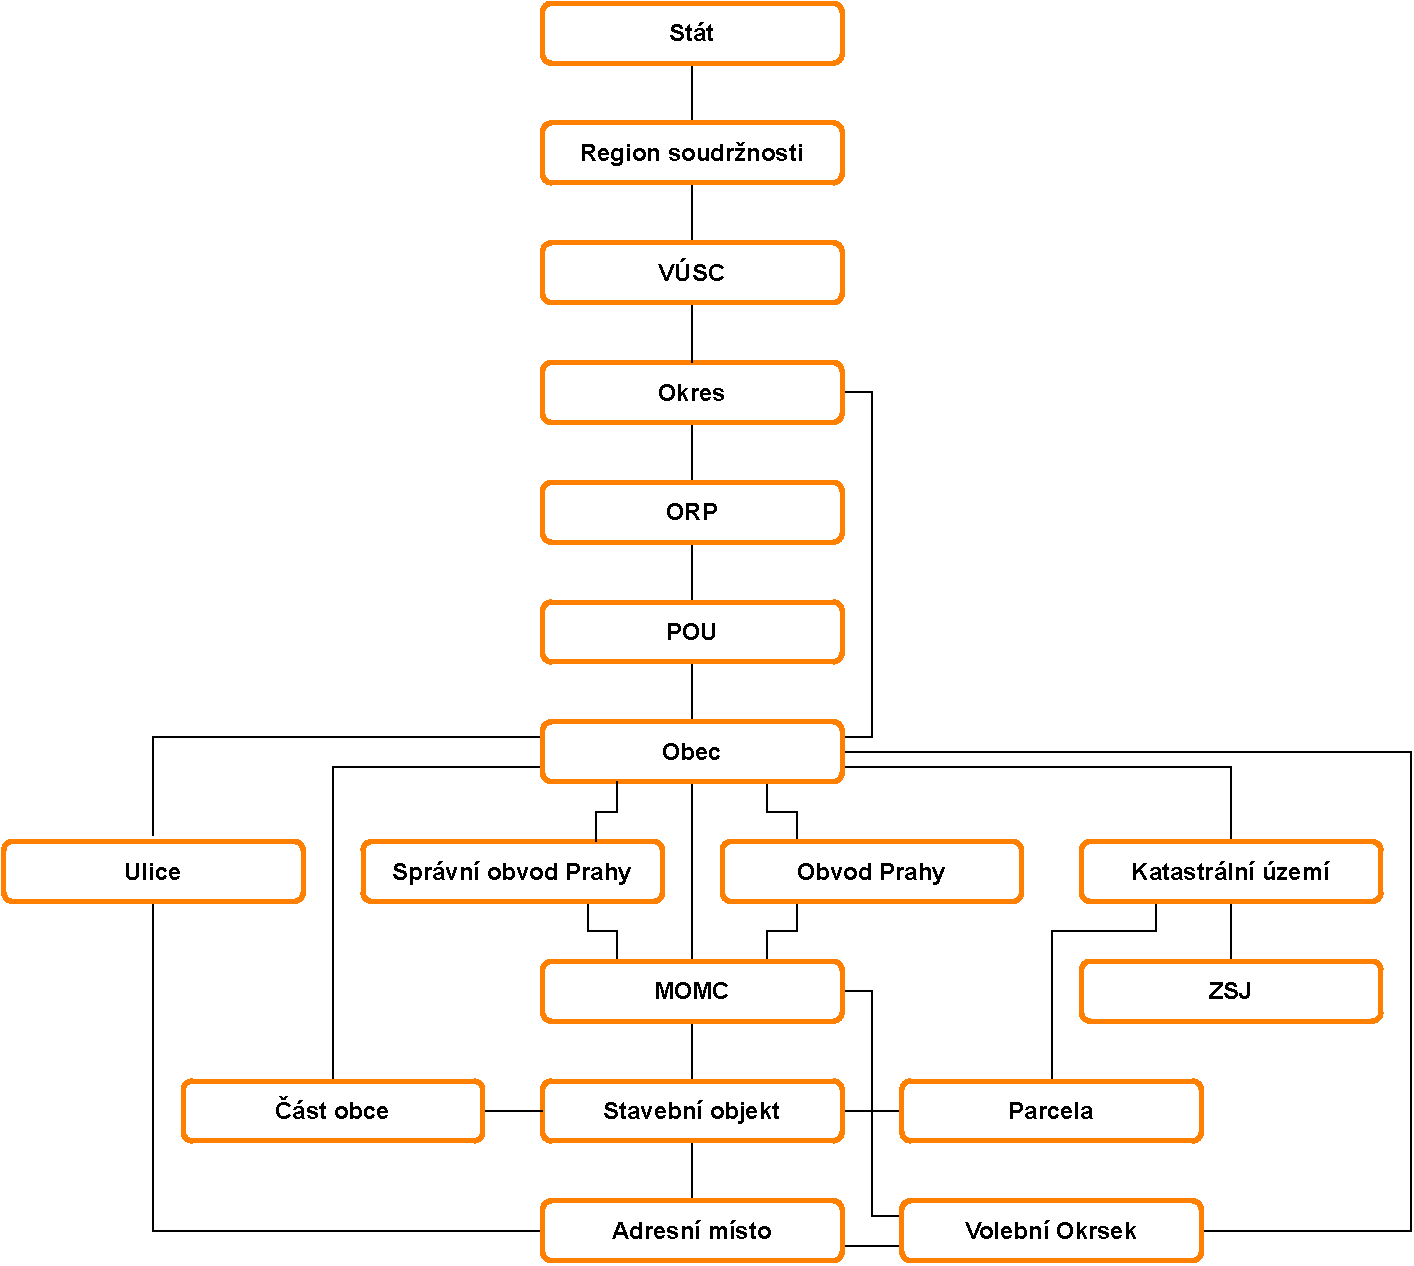
\includegraphics[width=\textwidth]{figures/ruian_diagram.pdf}
    \caption{Schéma prvků RÚIAN}
    \label{fig:ruian_tables}
\end{figure}

\newpage

\section{Formát dat}
Data z~RÚIAN jsou ve~formátu XML. Tento formát je strukturovaný a~umožňuje přenášet data mezi různými systémy.
Bude proto třeba implementovat parser, který převede data z~XML do~dále zpracovávaného formátu pro databáze.

Databázový systém je softwarový nástroj, který slouží k~efektivnímu ukládání, organizaci a~vyhledávání dat.
Díky své strukturované povaze umožňuje správu velkých objemů dat a~poskytuje funkcionality pro
zajištění konzistence, bezpečnosti a~rychlého přístupu k~uloženým informacím.

Databázový systém lze obecně rozdělit do~dvou hlavních kategorií: \textbf{relační} a~\textbf{objektový databázový systém}.
Každý z~těchto přístupů má své specifické vlastnosti a~je vhodný pro odlišné typy aplikací.

\subsubsection*{Relační databázové systémy}
\begin{itemize}[itemsep=-1pt]
    \item Data jsou uložena v~tabulkách.
    \item Každý řádek tabulky obsahuje jeden záznam.
    \item Každý sloupec tabulky obsahuje jeden atribut.
    \item Vztahy mezi tabulkami jsou definovány klíči.
    \item Využití jazyka SQL.
\end{itemize}
Relační databázové systémy jsou vhodné pro strukturovaná data, která mají pevnou strukturu.
Jedná se o~nejčastěji používaný typ databázových systémů.

\subsubsection*{Objektové databázové systémy}
\begin{itemize}[itemsep=-1pt]
    \item Data jsou uložena jako objekty.
    \item Každý objekt obsahuje atributy a~metody.
    \item Vztahy mezi objekty jsou definovány referencemi.
    \item Využití objektově orientovaného jazyka.
\end{itemize}
Objektové databázové systémy jsou vhodné pro nestrukturovaná data, která mají složitou strukturu.
Jedná se o~novější typ databázových systémů, který je vhodný pro moderní aplikace.

Vzhledem k~zadání, kde je přímo specifikováno, které databázové systémy budou použity,
není třeba vybírat mezi těmito dvěma systémy. Všechny tři databáze, které budou popsány,
jsou relační databázové systémy. Tyto systémy však mají mezi sebou rozdíly v~použití, funkcích a~možnostech.

Databáze bude potřebovat některé dodatečné funkce, které jsou nezbytné pro práci s~daty.
Mezi tyto funkce patří:
\begin{itemize}
    \item Zpracování geometrických dat.
    \item Podpora JSON.
    \item Podpora vhodných datových typů (čas a~datum, čísla, text).
\end{itemize}

\section{Microsoft SQL Server}
Microsoft SQL Server je relační databázový systém, který vyvinula společnost
Microsoft a~který se stal jedním z~předních nástrojů pro ukládání, správu a~analýzu dat.
SQL Server je robustní a~výkonný systém, který nabízí širokou škálu funkcí
a~možností přizpůsobení pro různé typy aplikací. Díky své dlouhodobé podpoře a~integraci
s~dalšími produkty společnosti Microsoft, jako je Azure nebo Power BI, je SQL Server
oblíbenou volbou pro velké a~střední podniky.

Edice SQL Serveru zahrnují Standard, Enterprise a~Express,
které se liší funkcemi a~cenou. Standard Edition je nejčastěji používanou edicí,
která obsahuje všechny základní funkce a~je vhodná pro většinu aplikací.

SQL Server byl původně navržen výhradně pro Windows, ale od verze SQL Server 2017 je dostupný
také pro operační systém Linux. Tato multiplatformní podpora zvyšuje jeho použitelnost
v~různých IT prostředích.
\cite{microsoft_sql_server}

Pro tuto práci bude využita edice SQL Server 2017 Standard, která je dostupná pro Windows a~Linux.
Tato edice podporuje vhodné datové typy pro zpracování geometrických dat.

\section{PostgreSQL}
PostgreSQL je open source relační databázový systém, který je známý svou spolehlivostí, výkonem
a~rozšiřitelností. Původně byl vyvinut jako alternativa k~proprietárním řešením, jako je SQL Server,
a~dnes se řadí mezi nejpokročilejší relační databázové systémy na trhu. Díky své otevřené povaze
a~aktivní komunitě uživatelů a~vývojářů se stal oblíbenou volbou nejen mezi malými firmami,
ale také ve středních a~velkých organizacích.

PostgreSQL je dostupný zdarma a~podporuje všechny hlavní operační systémy, včetně Windows, Linux a~macOS.
Tato multiplatformní dostupnost umožňuje snadnou integraci PostgreSQL do~různých vývojových prostředí.
\cite{postgresql}

PostgreSQL také podporuje jak formát JSON, tak všechny potřebné datové typy kromě geometrických dat.
Pro ukládání geometrických dat je třeba použít \textit{PostGIS}, což je rozšíření pro PostgreSQL, které přidává
podporu pro prostorové a~geometrické datové typy.

\section{Oracle Database}
Oracle Database, vyvinutá společností Oracle Corporation, patří mezi přední relační
databázové systémy na světě. Tento systém je známý svou robustností, vysokým výkonem
a~schopností zvládat kritické podnikové aplikace a~rozsáhlé datové sady. Oracle Database
je navržena tak, aby poskytovala spolehlivé a~efektivní řešení pro ukládání, správu
a~analýzu dat ve velkých i~středních organizacích.

Edice Oracle Database zahrnují Standard Edition, Enterprise Edition a~Express Edition,
které se liší funkcemi a~cenou. Enterprise Edition je nejkomplexnější edicí, která
obsahuje všechny pokročilé funkce a~je vhodná pro velké podniky s~náročnými požadavky.

Oracle Database je kompatibilní s~většinou hlavních operačních systémů, včetně Windows,
Linux a~Unix. Díky tomu může být nasazena v~různorodých IT prostředích podle požadavků organizace.
\cite{oracle_database}

Pro tuto práci bude využita edice Oracle Express Edition, která je dostupná zdarma a~je určena pro vývoj a~testování.
Tato edice podporuje všechny potřebné datové typy a~také JSON. Ovšem není zde možnost 
uložení geometrických dat. Ta jsou obsažena v~\texttt{SDO\_GEOMETRY}, což je rozšíření pro Oracle Database.

\section{Komunikace s~využitím SQL}
Všechny tři databázové systémy podporují dotazovací jazyk SQL (Structured Query Language).
SQL je standardizovaný jazyk pro práci s~relačními databázovými systémy, které umožňuje vytváření, čtení, aktualizaci a~mazání dat.
Pro komunikaci s~databází je tedy třeba vytvořit SQL dotazy, které budou provádět operace nad daty.
O~tuto komunikaci se stará aplikační vrstva, která zajišťuje připojení k~databázi a~následné zpracování a~odeslání SQL dotazů.

Vytvářet dotazy pro ukládání různých dat bude velmi náročné a~neefektivní.
Ve výsledné aplikaci bude použito ORM (Object-Relational Mapping), které umožňuje práci s~daty pomocí objektů.
ORM je technika, která mapuje objekty v~programovacím jazyce na tabulky v~databázi a~naopak.
Konkrétně bude použito \textit{Hibernate}, což je open-source ORM framework pro jazyk Java.

\section{JDBC}
Jedná se o~Java API pro přístup k~relačním databázovým systémům.
JDBC (Java Database Connectivity) poskytuje standardní rozhraní pro
připojení k~databázím a~použito pro připojení k~databázi a~provádění SQL dotazů.
Využívá různé ovladače pro různé databázové systémy, takže je možné připojit se k~jakékoli databázi,
která podporuje JDBC.
\chapter{Aplikace}
Aplikace je prostředníkem mezi RÚIAN VFR a cílovou databází.
Hlavním úkolem je stažení dat z~RÚIAN VFR, jejich přečtení, zpracování a následné uložení do cílové databáze.
Aplikace bude psána v~jazyce Java. Bude třeba zajistit funkce pro zpracování a uložení dat.

\section{Stahování dat}
Stahování dat bude zajištěno pomocí knihovny \textit{Apache HttpClient}, která je 
součástí balíčku \textit{Apache HttpComponents}. 
Tato knihovna umožňuje snadné a efektivní stahování dat z~webových stránek a API. 
V~rámci této aplikace bude použita k~stahování dat z~RÚIAN VFR.
Data budou stažena jako ZIP soubor, který bude následně rozbalen a zpracován.
Soubory budou uloženy do dočasného adresáře, který bude po zpracování smazán z~důvodu úspory místa na disku.

\section{Zpracování dat}
Zpracování dat se bude skládat z~několika částí:
přečtení a mapování dat do objektů, které budou následně uloženy do databáze.
Pro čtení dat bude třeba parser XML souborů, který přečte data a převede je do objektů.
Vzhledem k~velikosti dat bude třeba zajistit efektivní zpracování, aby nedocházelo 
k~přetížení paměti a CPU.
Pro čtení je možné využít knihovnu \textit{Jackson} nebo \textit{StAX}.

\begin{enumerate}
    \item \textbf{Jackson} -- knihovna pro zpracování JSON a XML dat. Umožňuje snadné mapování 
    objektů na JSON a XML a naopak. Je velmi rychlá a efektivní, ale může být složitější na použití.
    \item \textbf{StAX} -- knihovna pro zpracování XML dat. Umožňuje 
    čtení a zápis XML dat pomocí událostí. Je velmi rychlá a efektivní, ale může být 
    složitější na použití.
\end{enumerate}

\newpage

Následně bude třeba vytvořit objekty pro mapování dat do objektů.
Tyto objekty budou mít stejnou strukturu jako data z~RÚIAN VFR.
Pro mapování bude využita knihovna \textit{JPA} (Java Persistence API), která umožňuje snadné 
mapování objektů na databázové tabulky a naopak.
Pro tuto technologii je třeba vytvořit databázové entity, které budou mít stejnou strukturu jako
v~databázi. Dále bude třeba vytvořit repozitáře pro práci s~databází (CRUD operace).
A nakonec bude třeba vytvořit služby, které budou sloužit pro práci s~repozitáři a pro zpracování dat.

Před uložením do databáze bude třeba provést validaci dat, aby nedocházelo k~chybám při
ukládání. Je třeba zajistit, aby se zabránilo ukládání dat, která jsou neplatná nebo nekompletní.
Možné chyby při validaci dat:
\begin{itemize}
    \item Chybějící primární klíče
    \item Nevalidní cizí klíče
\end{itemize}

\section{Komunikace s~databází}
Pro ukládání dat je třeba se nejprve připojit k~databázi.
Pro připojení k~databázi bude použita knihovna \textit{JDBC} (Java Database Connectivity), která
umožňuje připojení k~různým databázím pomocí standardního API.
Pro jednotlivé databáze budou použity různé JDBC ovladače, které umožňují připojení k~vybraným databázím.

Pro připojení k~databázi bude třeba vytvořit konfigurační soubor, který bude obsahovat
informace o~připojení k~databázi.
\newpage

\section{Konfigurace}
Konfigurace neboli nastavení je důležitou součástí každé aplikace.
V případě této aplikace se jedná o~nastavení při jejím spuštění.

\subsection{Vhodný formát}
Je třeba zajistit, aby aplikace byla schopna načíst konfigurační soubor a~podle něj se správně nakonfigurovat.
Je tedy nutné zvolit vhodný formát tohoto souboru.
Existuje několik možností, z~nichž je třeba vybrat tu nejvhodnější:

\begin{itemize}
    \item \textbf{XML (XSD)} -- Extensible Markup Language
    \item \textbf{JSON} -- JavaScript Object Notation
    \item \textbf{YAML} -- YAML Ain't Markup Language
    \item \textbf{INI} -- Initialization File
\end{itemize}

\subsubsection*{XML}
\cite{cisco_xml_json_yaml}
XML je značkovací jazyk, na rozdíl od JSON a~YAML.
Jedná se o~textový formát, který však není tak snadno čitelný pro člověka jako JSON nebo YAML.
Podporuje víceúrovňovou strukturu a~komentáře.
Dále umožňuje použití schémat, což dovoluje definovat strukturu a~typy dat.
XML je však zbytečně složité a~náročné na čtení i~psaní.
Navíc je čtení velmi pomalé a~náročné na výkon.

\subsubsection*{JSON}
\cite{cisco_xml_json_yaml}
JSON je formát pro výměnu dat, který je snadno čitelný jak pro člověka, tak pro počítač.
Jedná se o~textový formát, který se často používá k~přenášení dat mezi serverem a~klientem.
Podporuje víceúrovňovou strukturu, ale nepodporuje komentáře.
Je však velmi rozšířený a~podporovaný většinou programovacích jazyků.
Čtení i~zápis dat je jednoduchý a~rychlý.

\subsubsection*{YAML}
\cite{cisco_xml_json_yaml}
YAML je formát pro serializaci dat, který je čitelností a~strukturovaností podobný JSON.
Oproti JSON podporuje komentáře.
Pro člověka však může být YAML složitější a~náročnější na psaní.
Rychlost čtení je srovnatelná s~JSON, ale zápis je pomalejší.

\subsubsection*{INI}
INI je formát konfiguračních souborů, který je snadno čitelný pro člověka.
Podporuje komentáře i~víceúrovňovou strukturu.
Je však často nejednotný a~obtížně se s~ním pracuje.
Používá se spíše pro jednodušší konfigurační soubory a~není vhodný pro složitější aplikace.

\subsection{Závěr výběru}
Vzhledem k~tomu, že aplikace bude obsahovat mnoho funkcionalit a~bude vyžadovat nastavení řady parametrů, je třeba zvolit vhodný formát.
Prozatímní verze aplikace si žádá formát, který bude čitelný, snadno rozšiřitelný a~dostatečně flexibilní.
Proto je nejvhodnější volbou formát \textbf{JSON}.
JSON je snadno čitelný a~zápis je přehledný, podporuje víceúrovňovou strukturu a~je široce rozšířený.
Přestože nepodporuje komentáře, lze jeho strukturu snadno pochopit a~rozšířit o~další parametry.
Zároveň je JSON podporován většinou programovacích jazyků, což zajišťuje snadnou integraci.

\section{Obsah konfiguračního souboru}
Konfigurační soubor bude obsahovat nastavení aplikace.
Jedná se o~nastavení databáze, aplikace, plánovače a~parametry pro stahování dat.
Konkrétně se jedná o:

\begin{enumerate}
    \item \textbf{Databáze} -- Nastavení připojení k~databázi:
    \begin{itemize}
        \item Typ databáze -- MSSQL, PostgreSQL, Oracle
        \item Connection string -- připojovací řetězec
        \item Uživatelské jméno -- přihlašovací jméno do databáze
        \item Heslo -- heslo do databáze
        \item Název databáze -- cílová databáze pro ukládání dat
    \end{itemize}

    \item \textbf{Nastavení plánovače} -- Nastavení plánovače, který bude stahovat data:
    \begin{itemize}
        \item Interval -- interval stahování dat
        \item Přeskočení -- možnost přeskočit naplánované stahování
    \end{itemize}

    \newpage

    \item \textbf{Parametry pro stahování dat} -- Parametry pro stahování dat z~webové služby:
    \begin{itemize}
        \item Seznam krajů -- výčet krajů, pro které se budou data stahovat
        \item Stahovat geometrii -- ANO/NE (např. kvůli absenci geometrických typů v~Oracle XE)
        \item Velikost commitů -- počet záznamů na jeden commit do databáze
        \item Konkrétní tabulky, sloupce a~způsob práce s~vybranými daty
    \end{itemize}
\end{enumerate}

Toto nastavení bude uloženo v~konfiguračním souboru, který bude načten při startu aplikace.
Bude tedy třeba vytvořit třídu, která zajistí načtení tohoto souboru a~zpracování jeho obsahu.
Některé technologie pro tuto práci již byly zmíněny (Java, JDBC, Hibernate atd.) v~sekci \ref{sec:komunikaceDB}.  
Pro účely této práce budou potřeba ještě další technologie, které umožní tvorbu aplikace.

\section{REST API}
REST API (Representational State Transfer Application Programming Interface) je architektonický  
styl pro návrh webových služeb, který umožňuje snadnou a~efektivní komunikaci mezi klientem a~serverem.  
Tento přístup se stal jedním z~nejrozšířenějších způsobů integrace aplikací díky své jednoduchosti,  
flexibilitě a~nezávislosti na platformě. REST API využívá standardní metody protokolu HTTP, jako jsou  
GET, POST, PUT a~DELETE, k~provádění různých operací s~daty.

REST API poskytuje ideální prostředí pro implementaci přenosu dat díky své flexibilitě a~schopnosti  
pracovat s~různými datovými zdroji. V~této práci bude kladen důraz na robustnost a~spolehlivost API,  
což zahrnuje zpracování chybových stavů, zabezpečení komunikace (například prostřednictvím HTTPS)  
a~optimalizaci výkonu.  
\cite{rest_api}

\section{Spring Framework}
Spring Framework je open-source framework pro vývoj aplikací v~jazyce Java.  
V~tomto frameworku bude vytvořena aplikace, která bude vše spojovat dohromady.  
Spring Framework obsahuje mnoho modulů, které usnadňují vývoj aplikací,  
jako například Spring Boot, Spring Data, Spring Security atd.  
Pro účely této práce bude využit modul Spring Boot, který umožňuje rychlé  
vytvoření aplikace s~minimální konfigurací.  
\cite{spring_framework}

\section{Maven}
Maven je nástroj pro správu projektů v~jazyce Java, který usnadňuje správu závislostí,
kompilaci a~nasazení aplikací. Jedná se o jednoduchý a~efektivní nástroj, který umožňuje
správu projektů pomocí XML konfiguračního souboru.
Konkrétně se jedná o~soubor \texttt{pom.xml}, který obsahuje informace o~projektu, 
jako jsou závislosti, pluginy a~další nastavení.
\cite{maven}

\section{Plánovač}
V~popisu, co bude obsahovat konfigurační soubor, bylo zmíněno, že~bude třeba zvolit plánovač.  
Plánovač je nástroj, který umožňuje spouštění úloh v~pravidelných intervalech.  
Výhodou plánovače je, že umožňuje automatické spouštění úloh bez nutnosti manuálního zásahu.  

Existuje několik možných plánovačů, které lze použít:
\begin{itemize}
    \item \textbf{Cron} -- Unix
    \item \textbf{Task Scheduler} -- Windows
    \item \textbf{Quartz} -- Java
    \item \textbf{Apache Airflow} -- Python
\end{itemize}

Všechny tyto plánovače umožňují spouštění úloh v~pravidelných intervalech.  
Pro účely této práce byl zvolen plánovač Quartz, který je napsán v~jazyce Java a  
je podporován Spring Frameworkem.  

Intervaly mohou být nastaveny v~cron notaci, což umožňuje velkou flexibilitu při plánování úloh  
(například každý den ve 3:00, každý týden v~pondělí v~8:00, každý měsíc první den ve 12:00 atd.).

\section{Docker}
Docker je open-source platforma pro vývoj, nasazení a~provoz aplikací.  
Umožňuje vytváření kontejnerů, které obsahují všechny potřebné závislosti pro běh aplikace.  

Pro každou databázi je třeba vytvořit instanci, která bude obsahovat potřebné tabulky, data  
a~klienta pro komunikaci a~práci s~databází. Toto je úloha jako stvořená pro Docker,  
který umožňuje vytvoření kontejneru s~databází, který bude obsahovat veškeré potřebné závislosti  
pro běh aplikace.  
\cite{docker}

\newpage

\section{Grafický klient pro správu databáze}
Klient pro komunikaci s~databází je nástroj, který umožňuje připojení k~databázi a~provádění dotazů.  
Je třeba vybrat klienta, který bude podporovat náhled do všech databází použitých v~této práci.

Možnosti jsou:
\begin{itemize}
    \item \textbf{DBeaver} -- open-source nástroj pro správu databází, který podporuje mnoho různých databází.
    \item \textbf{SQL Developer} -- nástroj pro správu databází Oracle.
    \item \textbf{Adminer} -- open-source nástroj pro správu databází, který může zároveň běžet v~Dockeru.
\end{itemize}

Všechny tyto nástroje umožňují připojení k~databázi a~provádění dotazů.  
Pro účely této práce byl zvolen DBeaver, který podporuje širokou škálu databází a~edice Community Edition je open-source.  
Zároveň umožňuje export dat z~databáze do různých formátů (CSV, Excel, JSON atd.).  
\cite{dbeaver}

\section{Log4j}
Log4j je open-source knihovna pro logování v~jazyce Java.
Umožňuje snadné a~efektivní logování událostí v~aplikaci.
Je možné nastavit různé úrovně logování (DEBUG, INFO, WARN, ERROR, FATAL) a~také různé výstupy 
(soubor, konzole, databáze atd.).
Tato technologie bude používána v průběhu vývoje aplikace pro logování událostí.
\cite{log4j}
\chapter{Implementace databází}

Každá databáze měla své problémy, ale všechny se nakonec podařilo vyřešit.  
V~následujících sekcích se podíváme na jednotlivé databáze a~jejich implementaci.

\section{PostgreSQL}

PostgreSQL se ukázala jako nejjednodušší databáze pro implementaci.  
Databáze běží na lokálním serveru v~Dockeru.  
Pro vytvoření byl stažen oficiální image z~Docker Hubu  
společně s~knihovnou PostGIS, která je potřebná pro práci s~geodaty.

\begin{lstlisting}[language=bash]
docker pull postgres:latest
\end{lstlisting}

Po stažení image byl následně vytvořen a~spuštěn kontejner pomocí docker-compose:

\begin{lstlisting}[language=bash]
docker-compose up -d
\end{lstlisting}

Databáze je inicializována skriptem `init.sql`, který vytvoří potřebné tabulky a~indexy.  
Tento skript byl napsán specificky pro databázi PostgreSQL a~pomocí něj je vytvořena databáze  
se všemi potřebnými tabulkami.

\section{Microsoft SQL Server}

Microsoft SQL Server byla druhá databáze, která byla implementována.  
Při stahování oficiálního image z~Docker Hubu se objevily problémy.  
Po úspěšném stažení image `mssql/server:2017` byl kontejner spuštěn stejně jako u~PostgreSQL  
pomocí docker-compose.

Menším rozdílem je způsob spouštění `init` skriptu, který se nespouští při inicializaci databáze  
přes `entrypoint`, ale až následně pomocí příkazu `sqlcmd`.

\section{Oracle}

Oracle byla poslední databáze, která byla implementována.  
Při stahování oficiálního image z~Docker Hubu došlo k~problémům.  
Když se však image podařilo stáhnout a~kontejner spustit, databáze nefungovala správně.  
Nezbývalo nic jiného než stáhnout Oracle XE z~oficiálních stránek a~nainstalovat ho na lokální stroj.  
%TODO: popsat, jak se to instaluje a co to obnáší

\newpage

\section{Rozdíly ve skriptech pro jednotlivé databáze}

Každá databáze měla vlastní skript pro inicializaci databáze.  
Hlavní rozdíl byl v~syntaxi SQL příkazů.

\renewcommand{\arraystretch}{1.3}
\begin{table}[ht]
\centering
\caption{Datové typy v různých databázích}
\label{tab:datove_typy}
    \begin{tabular}{|l|l|l|l|}
        \hline
         & \textbf{Oracle} & \textbf{PostgreSQL} & \textbf{MSSQL} \\ \hline
        \textbf{Integer}     & NUMBER           & INTEGER           & INT               \\ \hline
        \textbf{Long}        & NUMBER(19)       & BIGINT            & BIGINT            \\ \hline
        \textbf{DateTime}    & DATE             & TIMESTAMP         & DATETIME          \\ \hline
        \textbf{String}      & VARCHAR2(length) & VARCHAR(length)   & NVARCHAR(length)  \\ \hline
        \textbf{JSON}        & JSON             & JSONB             & NVARCHAR(MAX)     \\ \hline
        \textbf{Boolean}     & NUMBER(1)        & BIT               & BIT               \\ \hline
        \textbf{Geometry}    & SDO\_GEOMETRY    & GEOMETRY          & GEOMETRY          \\ \hline
        \textbf{Binary}      & BLOB             & BYTEA             & VARBINARY         \\ \hline
    \end{tabular}
\end{table}

Velkým rozdílem byly také cizí klíče (foreign key), které byly v~každé databázi definovány odlišně.

\begin{itemize}
    \item \textbf{PostgreSQL}:
    \begin{lstlisting}[language=sql]
<column_name> INTEGER REFERENCES <table>(<column_name>)
<column_name> BIGINT REFERENCES <table>(<column_name>)
    \end{lstlisting}

    \item \textbf{MSSQL}:
    \begin{lstlisting}[language=sql]
<column_name> INT FOREIGN KEY REFERENCES 
    <table>(<column_name>)
<column_name> BIGINT FOREIGN KEY REFERENCES 
    <table>(<column_name>)
    \end{lstlisting}

    \item \textbf{Oracle}:
    \begin{lstlisting}[language=sql]
<column_name> <column_type>,
CONSTRAINT <constraint_name> FOREIGN KEY (<column_name>) 
    REFERENCES <table>(<column_name>)
    \end{lstlisting}
\end{itemize}
\chapter{Implementace aplikace}
Před začátkem popisu implementace aplikace je dobré říct, o co se aplikace bude snažit.
Cílovým účelem aplikace je stahování dat z~API RÚIAN a jejich následné zpracování.
Výsledkem bude projekce dat do databáze, která bude následně použita pro další zpracování.
Aplikace bude napsána v~programovacím jazyce Java a~použije framework Spring Boot.

\section{Projekce databáze}
Projekce databáze je způsob zobrazení dat z jedné databáze do druhé databáze.
Podle konfigurace se nastaví úroveň projekce a~podle toho se budou zobrazovat data.
Nastavení projekce bude dále popsáno v~sekci \ref{sec:konfigurace}.

\section{Inicializace aplikace}
Na začátku aplikace se provede její inicializace.
Důvod, proč byl vybrán právě framework Spring Boot, je funkčnost aplikace spočívající v~automatickém načtení všech komponent a~konfigurací.
Konkrétně se jedná o~moduly označené anotacemi @Component, @Service, @Configuration, @Entity, @Repository a~@Bean.

\subsection{Připojení k databázi}
O připojení k~databázi se stará třída \texttt{DatabaseSource}, která je zodpovědná za navázání spojení s databází.
Z konfiguračního souboru se načtou potřebné informace pro připojení k databázi.
Konkrétně se jedná o~tyto informace:
\begin{itemize}
    \item \texttt{type} -- typ databáze (např. \texttt{postgresql}, \texttt{mssql}, \texttt{oracle})
    \item \texttt{url} -- adresa databáze (např. \texttt{localhost:5432} pro PostgreSQL)
    \item \texttt{dbname} -- název databáze (např. \texttt{ruian})
    \item \texttt{username} -- uživatelské jméno pro připojení k databázi
    \item \texttt{password} -- heslo pro připojení k databázi
\end{itemize}

Podle těchto informací se vytvoří připojení k databázi, neboli \textbf{DataSource}.
\texttt{DataSource} slouží jako zdroj dat pro JPA a~je zodpovědný za správu spojení s databází.
Tento zdroj bude dále upraven v jiném modulu.
Základem \texttt{DataSource} je nastavení prvotních parametrů připojení.
Vytváří se tedy výsledný connection string, který se modifikuje podle typu databáze.
K URL se připojí název databáze, uživatelské jméno, heslo, a~v případě MSSQL se přidává i certifikát pro zabezpečené připojení.

V dalším modulu se pro \texttt{DataSource} donastavují další parametry pro přístup k databázi a~přenos dat.
Jako první se inicializují DTO objekty, repozitáře a~třídy typu \texttt{Service} pro JPA.
Tyto objekty se inicializují pomocí anotace \texttt{@Autowired}, která je zodpovědná za injektování závislostí.
Dále se nastaví dialekt pro správnou syntaxi SQL příkazů podle dané databáze.

\subsection{Načtení konfigurace}
\label{sec:konfigurace}
Zatímco \texttt{DatabaseSource} se stará pouze o~nastavení a připojení k databázi,
třída \texttt{AppConfig} se stará o~načtení zbytku informací.
Konfigurace se načítá následovně:
\begin{enumerate}
    \item Konfigurace úkolů pro \texttt{Quartz Scheduler}. 
    Konkrétně se načítá čas ve formátu cron pro spouštění přidávání přírůstkových dat.
    Dále se načítá informace, zda přeskočit základní inicializaci pro hlavní územní prvky a kraje.
    
    \item Seznam krajů s příslušnými kódy. Každý řádek v konfiguračním souboru obsahuje kraj s jeho kódem.
    Pokud je v konfiguraci pro \texttt{Quartz Scheduler} nastaveno přeskočení inicializace krajů nebo je seznam prázdný,
    tento krok je zcela přeskočen.
    
    \item Dodatečná nastavení. Především se jedná o~nastavení pro ignorování geometrických dat.
    Toto je implementováno z~důvodu, že některé databáze nepodporují geometrické datové typy.
    Dále je zde nastavení velikosti jednotlivých commitů do databáze, což je prvek optimalizace výkonu.
    
    \item Nastavení zpracování jednotlivých tabulek. Hlavním parametrem je způsob zpracování tabulek, který může být
    \texttt{all} nebo \texttt{selected}. Pokud je nastavení \texttt{all}, budou zpracovány všechny tabulky bez ohledu na další konfiguraci.
    
    \begin{itemize}
        \item \textbf{all} -- všechny tabulky budou zpracovány bez ohledu na konfiguraci jednotlivých tabulek.
        \item \textbf{selected} -- budou zpracovány pouze tabulky, které jsou výslovně uvedeny v konfiguraci.
    \end{itemize}
    
    \item Konfigurace jednotlivých tabulek. Pokud je nastaven režim \texttt{selected}, zpracovávají se jen specifikované tabulky.
    Každá tabulka může mít své vlastní nastavení:

    \begin{lstlisting}[language=json, caption=Konfigurace tabulek, label=lst:konfTabulek]
"<table_name>": {
    "howToProcess": "all | exclude | include",
    "columns": ["<column_name>", ..., "<column_name>"]
}
    \end{lstlisting}

    Možnosti zpracování tabulky:
    \begin{itemize}
        \item \textbf{all} -- všechny sloupce budou zpracovány bez ohledu na konfiguraci.
        \item \textbf{exclude} -- vybrané sloupce budou ignorovány, ostatní budou zpracovány.
        \item \textbf{include} -- vybrané sloupce budou zpracovány, ostatní budou ignorovány.
    \end{itemize}

    Sloupce jsou definovány jako pole řetězců s názvy sloupců.
\end{enumerate}

Možné chyby při načítání konfigurace:
\begin{itemize}
    \item Pokud je u tabulky nastaveno \texttt{exclude} nebo \texttt{include}, ale nejsou uvedeny žádné sloupce \textrightarrow{} nevalidní konfigurace.
    \item Sloupce nebo tabulky, které neexistují v databázi \textrightarrow{} budou přeskočeny a~nebudou zpracovány.
    \item Seznam krajů je povinný atribut, i pokud je prázdný. Pokud je prázdný, budou zpracovány pouze základní územní prvky.
\end{itemize}

\newpage

\section{Quartz Scheduler}
\subsection{Jobs}
\subsection{Triggers}

\section{Stahování dat}
\subsection{Stahování dat z~API}

\section{Zpracování dat}
\subsection{Dto objekty}
\subsection{Repositáře}
\subsection{Service třídy}
\subsection{Parsing dat}
\subsection{Validace dat}
\subsection{Ukládání dat do databáze}
\section{Rychlostní porovnání databázových systémů}
Tento test byl proveden na stejném konfiguračním souboru pro všechny databázové systémy.
Testovací konfigurace je nastavena na provedení stažení, zpracování a~uložení Základní datové sady Stát~až~ZSJ.
Tato datová sada byla vybrána z důvodu neměnnosti. 
Data v této datové sadě se mění jen velmi zřídka a~je možné je stáhnout.
Dále bylo nastavené, že se zpracují všechny tabulky uvedené v~již zmíněné datové sadě.
Geometrie bude zpracována a~velikost jednotlivých commitů bude 2000.
Vzhled konfiguračního souboru je uveden v~příkladu \ref{lst:konfigTest} a~bude konfigurován pro PostgreSQL.
Testování probíhalo na stejném stroji, který měl instalované všechny databázové systémy.

Nad všemi databázovými systémy probíhaly testy \(3\times\), aby se eliminovaly chyby způsobené jinými procesy na serveru.
Každý test byl proveden na prázdné databázi.
Měření začalo, když byla data připravena ke čtení z důvodu eliminace stahování dat z~internetu.
Konkrétně když se vypsala zpráva \uv{Data proccesing started.} a~následně skončilo, když se 
vypsala zpráva \uv{Data proccesing finished.}.
Během tohoto testu byl také vyfiltrováno 1 ZSJ z důvodu neexistence cizího klíče v~tabulce Katastrální území.
Testování proběhlo s daty \url{https://vdp.cuzk.gov.cz/vymenny_format/soucasna/20250331_ST_UZSZ.xml.zip}
Výsledky jsou uvedeny v~tabulce \ref{tab:test1} a mají formát HH:MM:SS.

\begin{table}[!h]
  \centering
  \caption{Časy testů pro používané databáze}
  \label{tab:test1}
  \begin{tabular}{|c|c|c|c|}
  \hline
                  & \textbf{PostgreSQL} & \textbf{MS SQL} & \textbf{Oracle} \\ \hline
  \textbf{test 1} & 0:35:59             & 0:22:46         & 1:04:19         \\ \hline
  \textbf{test 2} & 0:37:03             & 0:22:26         & 1:05:30         \\ \hline
  \textbf{test 3} & 0:35:53             & 0:21:26         & 1:04:57         \\ \hline
  \textbf{průměr} & 0:36:18             & 0:22:13         & 1:04:55         \\ \hline
  \end{tabular}
\end{table}

Jak je vidět v tabulce \ref{tab:test1}, ukázalo se že MS SQL je nejrychlejší databázový systém pro zpracování datové sady.
PostgreSQL je o~přesně 14 minut pomalejší než MS SQL a~Oracle je o~přesně 28 minut pomalejší než MS SQL.
Je ale možné že Oracle je pomalejší z důvodu že se jedná o~Express verzi, která je omezena na 2GB RAM a~1 CPU.
Dále je možné že rychlost byla omezena prostředím. Zatím co PostgreSQL a MS SQL běžely v Docker kontejneru, 
Oracle běžel přímo na hostitelském systému.

\begin{lstlisting}[language=json, caption={Konfigurační soubor pro test rychlosti}, label={lst:konfigTest}]
    {
        "database": {
          "type": "postgresql",
          "url": "jdbc:postgresql://localhost:5432",
          "dbname": "ruian",
          "username": "postgres",
          "password": "123"
        },
        "quartz": {
          "cron": "0 0 2 * * ?",
          "skipInitialRunStat": false,
          "skipInitialRunRegion": true
        },
        "vuscCodes": {},
        "additionalOptions": {
          "includeGeometry": true,
          "commitSize": 2000
        },
        "dataToProcess": {
          "howToProcess": "all"
        }
      }    
\end{lstlisting}


\section{Testování kompletního importu}

Na této aplikaci je stále co přidávat, vylepšovat a~upravit.
Proto se v následujících sekcích pokusím shrnout, co by se 
dalo do budoucna vylepšit a přidat.

\section*{Uživatelské rozhraní}
Jediný uživatelský pohled na aplikaci je v~současnosti zajištěn pomocí 
logu, který je generován v~textovém formátu. Jedná se pouze o výpis
informací o~prováděných úkonech, které aplikace dělá.
Bylo by dobré přidat uživatelské rozhraní, které by bylo schopné
zobrazit informace o~prováděných úkonech v~reálném čase.


\section*{Optimalizace}
Aplikace je v~současnosti napsána tak, že se snaží aby byla schopná
zpracovat jakákoliv data z~RÚIANu. Ovšem rychlostně to není
úplně ideální. Hlavním kamenem úrazu je především kontrola
a~porovnání nových dat s~těmi, které jsou už v~databázi.
Bylo by dobré nějak zefektivnit tento proces, aby se obecně zrychlil
celý proces zpracování dat.

\section*{Refektoring kódu}
Tenhle oddíl vzchází trochu z~předchozího. Aplikace je napsána
tak aby byla schopná zpracovat jakákoliv data z~RÚIANu.
Bylo bz proto dobré udělat refaktoring kódu, aby se zjednodušil
a zefektivnil celý proces zpracování dat. Service třídy, Dto 
by se určitě upravit pomocí nějakého generického rozhraní.
Využití abstraktních tříd a~rozhraní by mělo celý kód velmi
zjednodušit.

\section*{Zpracování zbylých dat}
V současnosti aplikace zpracovává pouze základní datové sady.
To znamená zpracování zbývajících geometrických dat, které jsou
v~RÚIANu k~dispozici. Dále zakomponovat obrázky (binární data),
které se u některých objektů vyskytují.
Databáze je v~současnosti připravena na zpracování těchto dat,
ale aplikace nemá implementovanou logiku pro jejich zpracování.

\section*{Podpora pro dalších databázových systémů}
Rozšíření aplikace o~další databázové systémy by bylo mohla
býti samozřejmostí. V~současnosti je aplikace napsána tak,
že je schopná pracovat pouze s~PostgreSQL, MS SQL a~Oracle databázemi.
Bylo by dobré přidat podporu pro další databázové systémy.
Hlavním cílem této bakalářské práce bylo vytvořit aplikaci, která by byla
schopná stahovat data podle konfigurace z~RÚIANu a~ukládat je do databáze.
V rámci práce jsem navrhl prvotní verzi aplikace, která splňuje tento cíl,
implementoval jsem ji a~otestoval jsem ji na vzorových datech z~RÚIANu
pro všechny zadané databázové systémy.

Vytvořená aplikace je první verze aplikace se jménem \textbf{Ruian\_Puller},
která má za úkol stahovat data z~RÚIANu a~ukládat je do databáze.
Podporované databáze jsou PostgreSQL, MySQL a~Oracle.
Aplikace je napsaná v~programovacím jazyce Java a~využívá framework Spring Boot.
Je možné použití plánování úloh pomocí Quartz Scheduleru.
Aplikace se nastavuje podle konfiguračního souboru,
který je ve formátu JSON. Nastavuje se připojení k databázi,
jaké prvky se mají stahovat, či ignorovat a~jak často se stahování má provádět.
Aplikace je navržena jako základ pro budoucí rozšíření a úpravy (viz kapitola~\ref{cha:NavrhDoBudoucna}).
 
%---------------------------------------------------------------------------
\appendix
\chapter{První příloha}
\backmatter
\printbibliography
\setbackpageqrcode
\backpage
\end{document}